\documentclass{beamer}

\usepackage{graphicx}

\begin{document}
%---------------------------------------------------------------------------%

\frame{
\frametitle{Boxplots}
\begin{itemize}
\item A graphical method we will be looking at today is the `box-and-whisker' plot (commonly just referred to as `boxplots')
\item The boxplots is a useful tool for assessing the distribution of a dataset, by means of a visual summary.
\item consider the data set of the exam scores of 100 students (see next slide).
\item The quartiles of the data set were $Q_1 = 42.5$, $Q_2 = 54.5$ (with $Q_2$ being the median), and $Q_3 =  65.5$ respectively.
\item The interquartile range is $Q_3 - Q_1 = 23$
\item The boxplot of the distribution is featured on the second next slide.
\end{itemize}
}
%---------------------------------------------------------------------------%
\frame{
\begin{table}[ht]
\caption{Exam results of 100 students} % title of Table
\centering % used for centering table
\begin{tabular}{|c ccc ccc ccc|} % centered columns (4 columns)\hline
\hline

13	&	21	&	22	&	23	&	24	&	25	&	26	&	28	&	29	&	30	\\	31	&	32	&	33	&	34	&	35	&	 36	&	36	&	36	&	37	&	38	\\
39	&	41	&	41	&	41	&	42	&	43	&	44	&	44	&	44	&	45	\\	45	&	46	&	47	&	49	&	50	&	 51	&	51	&	52	&	53	&	53	\\
53	&	53	&	53	&	54	&	54	&	54	&	54	&	54	&	54	&	54	\\	55	&	55	&	55	&	56	&	56	&	 56	&	57	&	57	&	58	&	59	\\
62	&	63	&	63	&	63	&	63	&	64	&	64	&	64	&	64	&	64	\\	65	&	65	&	65	&	65	&	65	&	 66	&	66	&	66	&	67	&	69	\\
71	&	71	&	72	&	72	&	73	&	74	&	75	&	76	&	76	&	76	\\	77	&	82	&	84	&	85	&	87	&	 88	&	91	&	91	&	92	&	99	\\ \hline
\end{tabular}
\end{table}
}
%--------------------------------------------------------%

\frame{
\frametitle{Boxplots}

\begin{center}
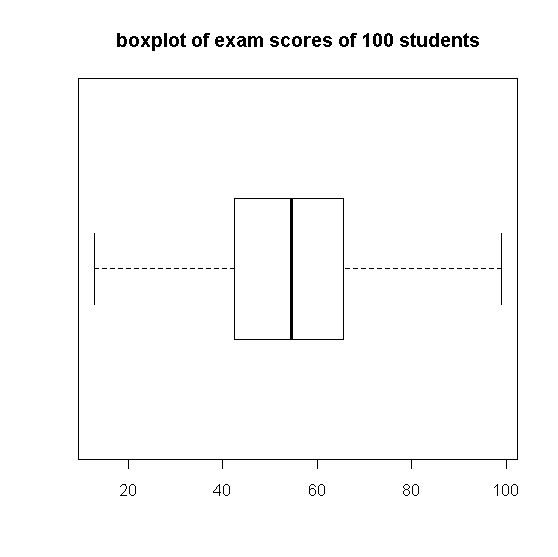
\includegraphics[scale=0.40]{images/3Bboxplot1}
\end{center}
}

%--------------------------------------------------------%
\frame{
\frametitle{Boxplots}
\begin{itemize}
\item The boxplot is a visual summary containing important aspects of a distribution. \item The main component of the plot , the `\textbf{\emph{box}}', stretches from the \textbf{\emph{lower hinge}}, defined as $Q_1$, to the \textbf{\emph{upperhinge}}, defined as $Q_3$ .
\item (\textbf{Important:}) The median is shown as a line across the box.
\item Therefore the box contains the middle half of the scores in the distribution.
\item  1/4 of the distribution is between the median line and the upper hinge. Similary 1/4 of the distribution is between the median line and the lower hinge.
\end{itemize}
}

\begin{frame}
	\begin{figure}
Boxplot (No Outliers Present)
\centering
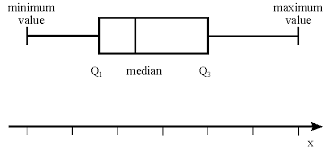
\includegraphics[width=0.9\linewidth]{images/boxplotstructure}
\caption{Structure of Boxplots}

\end{figure}

\end{frame}
\frame{
	\frametitle{Boxplots}
	\begin{itemize}
		\item Any value considered to be an outlier should be indicated with an asterisk or a small circle.
		\item We will see an example of a boxplot with outliers on the next slide.
	\end{itemize}
	
	
}
\begin{frame}
Boxplots can be used to indicate presence of outliers.
	\begin{figure}
\centering
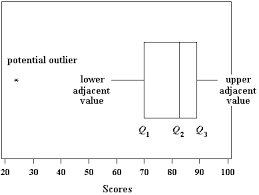
\includegraphics[width=0.85\linewidth]{images/boxplotstructure2}
\end{figure}

\end{frame}
%---------------------------------------------------------------------------%
\frame{
\frametitle{Boxplots}
\begin{itemize}
\item On either side of the box are the \textbf{\emph{whiskers}}.
\item To find where to place the whiskers, we must first compute the location of the \textbf{\emph{fences}}, and determine whether or not there are any \textbf{\emph{outliers}} present.
\item Firstly, we must compute the location of the \textbf{\emph{lower fence}}.
\[ \mbox{ Lower Fence}  = Q_1 - 1.5 \times IQR \]
\item For our example, the lower fence is
\[ \mbox{ Lower Fence}  = 42.5 - 1.5 \times 23  = 42.5 - 34.5 = 8 \]
\item \textit{(Fences were called adjacent values on diagram on previous slide)}
\end{itemize}
}
%---------------------------------------------------------------------------%
\frame{
\frametitle{Boxplots}
\textbf{Detecting Outliers} \\
\begin{itemize}
\item The lower fence is used to determine whether there are any outliers in the lower half of the data set.
\item \textbf{Important:} If there is any observed value less than the lower fence, it is considered an outlier.
\item \textbf{Important:} The first whisker is drawn at the location of the lowest value that is not considered an outlier.
\item If no values are considered outliers, then the whisker is drawn at the location of the smallest value of the dataset.
\item For our dataset, the lowest value is 13, which is not less than the lower fence.
\item Therefore we draw the first whisker, a vertical line, at this location. A horizontal line is drawn connecting the location of this whisker to $Q_1$.
\end{itemize}
}

%---------------------------------------------------------------------------%
\frame{
\frametitle{Boxplots}
\begin{itemize}
\item Now we must compute the location of the \textbf{\emph{upper fence}}.
\[ \mbox{ Upper Fence}  = Q_3 + 1.5 \times IQR \]
\item For our example, the upper fence is
\[ \mbox{ Upper Fence}  = 65.5  + 1.5 \times 23  = 65.5 + 34.5 = 100 \]
\end{itemize}
}
%---------------------------------------------------------------------------%
\frame{
\frametitle{Boxplots}
\begin{itemize}
\item The upper fence is used to determine whether there are any outliers in the upper half of the data set.
\item If there is any observed value greater than the upper fence, it is considered an outlier.
\item The second whisker is drawn at the location of the highest value that is not considered an outlier.
\item If no values are considered outliers, then the whisker is drawn at the location of the highest value of the dataset.
\item For our dataset, the highest value is 99, which is less than the upper fence.
\item Therefore we draw the second whisker , a vertical line, at this location.
\item A horizontal line is drawn connecting the location of this whisker to $Q_3$.
\end{itemize}
}
%---------------------------------------------------------------------------%
\frame{
\frametitle{Boxplots}
\begin{itemize}
\item Remark: If you do not get a sensible value for either the upper or lower fence, you can replace it with the nearest sensible value
\item For example, suppose we got a negative lower fence value. It does not make sense to get a negative score in an exam.
\item In this case, we could replace the value with a value of $0$.
\item Similarly for the upper fence: any fence value greater than 100 should be replaced with the value of 100.
\end{itemize}
}
%---------------------------------------------------------------------------%
\frame{
\frametitle{Boxplots}
\large
\begin{itemize}
\item Boxplots are very useful in comparing the distributions of two or more groups when measured by the same variable.
\item They can be used to assess how similar the centrality of the various groups. ( also called ``location").
%\item Recall the experiment of 60 students, each throwing a die 100 times.
%\item Suppose they perform this experiment twice, firstly with a fair die, and then with a crooked die.
%\item (The probability of the outcomes from the crooked die are as per yesterday's class).
\item Boxplots can use used to compare the dispersion of scores for all of these groups. ( also called ``scale").
\end{itemize}
}

%--------------------------------------------------------%

\frame{
\frametitle{Boxplots}
Groups A,C,E have similar centrality. Group B and D has similar centralities also, but different from A,C and E. The dispersion is roughly the same for each group.
\begin{center}
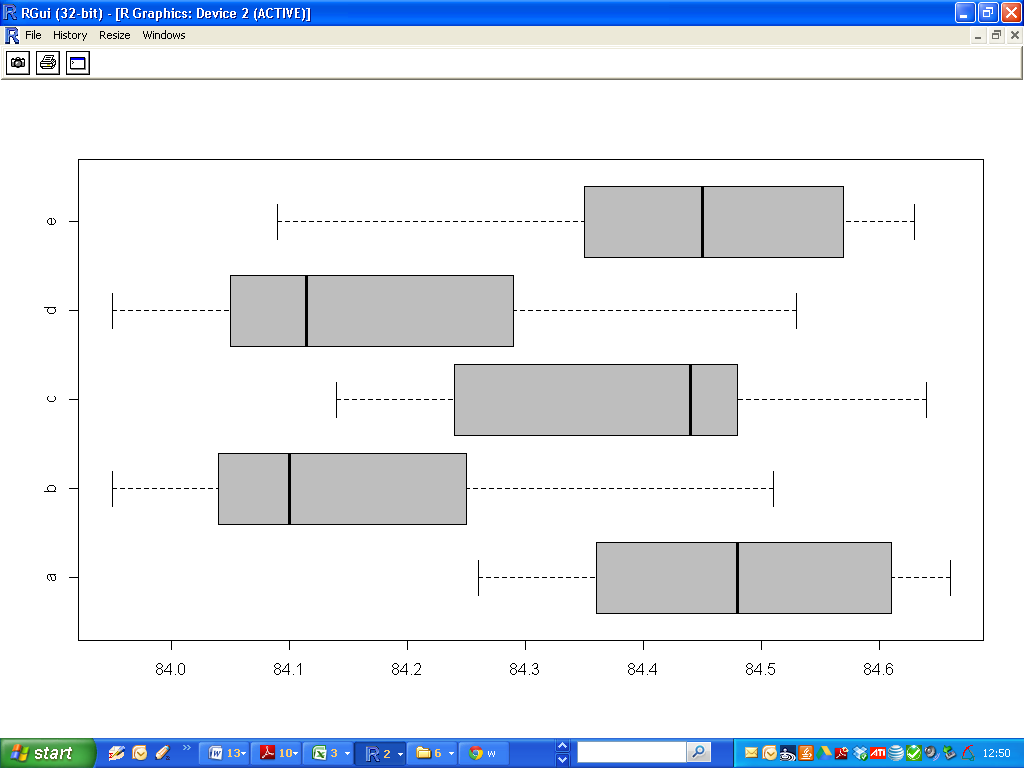
\includegraphics[scale=0.240]{images/Boxplot2}
\end{center}
}

%--------------------------------------------------------------------------------------%
%--------------------------------------------------------%

\frame{
Much higher dispersion indicated for Group F (top group). \\ Other groups have similar dispersion (``scale").
	\frametitle{Boxplots}
	
	\begin{center}
		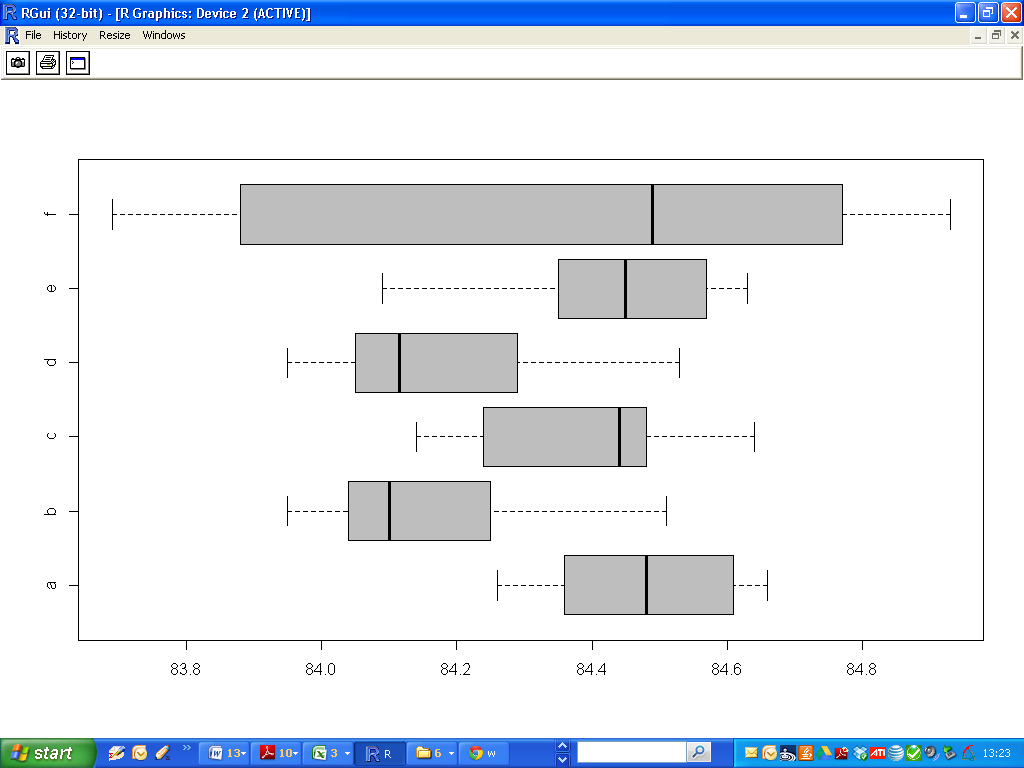
\includegraphics[scale=0.250]{images/Boxplot3}
	\end{center}
}
\begin{frame}
	\textbf{Review}
	\Large
\begin{itemize}
	\item Be able to interpret a box-plot, particularly for indicating outliers.
	\item Know the procedure used to determine if a point should be considered an outlier  (i.e. comparing values to Lower and Upper Hinges)
	\item Use boxplots to compare scale and location for different groups.
\end{itemize}
		
\end{frame}
\end{document}